    \documentclass[11pt]{article}
    %	options include 12pt or 11pt or 10pt
    %	classes include article, report, book, letter, thesis
    
    \title{HW4}
    \author{Shane Drafahl}
    \date{16 October ,2017}
    \usepackage{graphicx}
    \usepackage{epstopdf}
    \usepackage{graphics}

    \begin{document}
    \maketitle

    1. $ \newline \newline $

    \begin{figure}[!htb]
        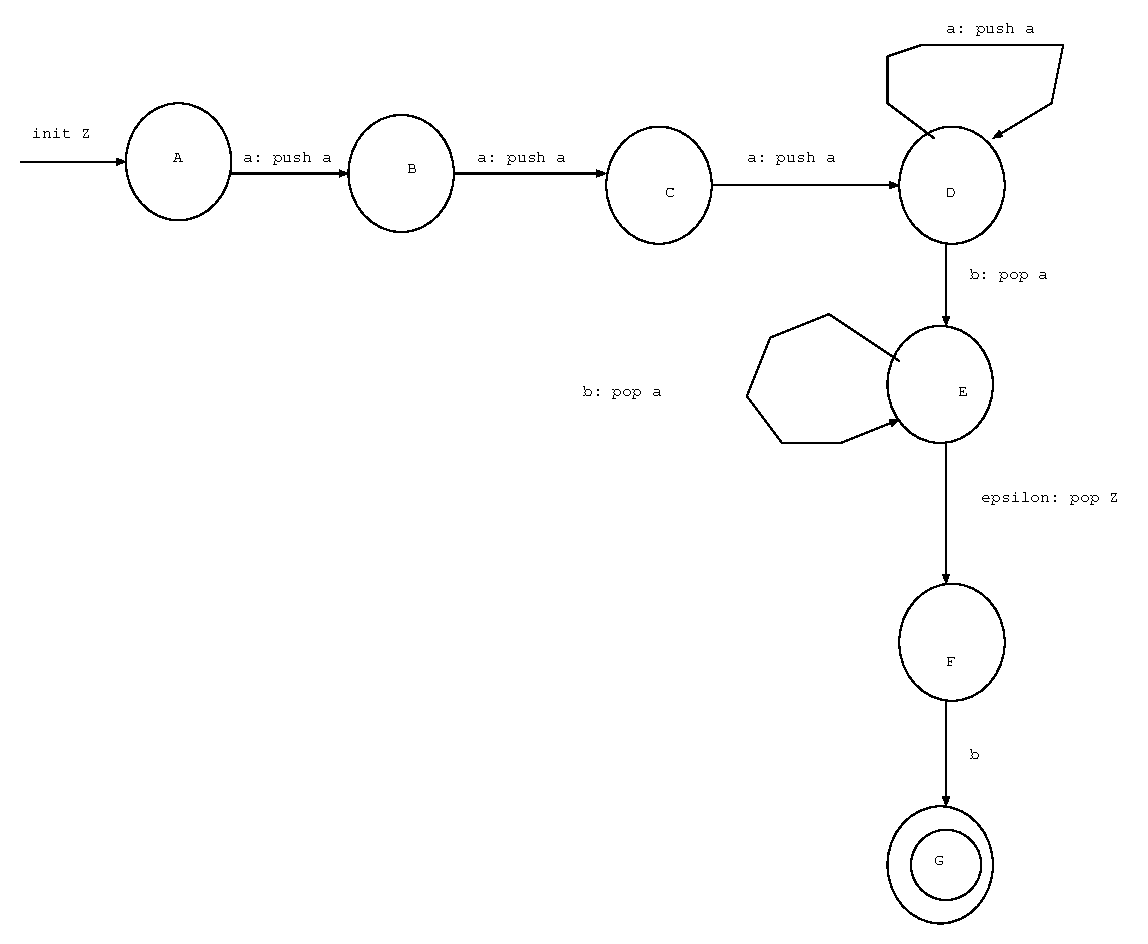
\includegraphics[scale=.6]{./hw8_1.eps}
    \end{figure}

    $ \newline $

    2.

    $ \newline $

    By contradiction if we assume that this language is context-free. So
    there would be an m such that any string $ w \in L $, $ |w| \geq m $. 
    We will choose w = $ b^{m}a^{m+1}b^{m} $. w cannot be decomposed into w = $ uv^{k}xy^{k}z $ where 
    k is a natural number.
    $ \newline $
    case 1: vxy are composed of all a's. If k = 0 then there will be at least one less a meaning that at least the
    longest run of a's and b's would be equal or the longest run of b's would be longer.
    $ \newline $
    case 2: vxy are composed of all b's. If k = 1 then at least there would be one additional b. Meaning  that at least the 
    longest run of a's and b's would equal otherwise the longest run of b's would be longer.
    $ \newline $
    case 3: vxy are compose of a's and b's. vxy cannot be greater than m so either the middle and left 
    run or the middle and right run can be pumped at most. Also because of the restriction 
    that v and y cannot be both epsilon we know that we will either pump just b's , just a's or both a's and b's.
    If we pump just a's or just b's k = 1 for just b's and k = 0 for just a's similar to case 1 and 2. Otherwise if 
    we pump both a's and b's if k = 0 then there will be one less a or b in either of the runs. This will mean one of the 
    runs of b's will now be equal or longer than the runs of a's.

    $ \newline $

    3. With proof by contradiction we will assume L is context-free. Therefore we can use closure properties 
    such as reversal to get $ L^{'} = L^{R} $. We will then concatinate $ L^{''} = L L^{'} = a2bb^{R}2a^{R} $.
    We will then do a pumping lemma on $ L^{''} $. So there would be an m such that any string $ w \in L $, $ |w| \geq m $.
    we will choose w = $ 1^{m}210^{m}0^{m}121^{m} $. If we split this up with $ uv^{k}xy^{k}z $ where k is a natural number.
    The only way this can be pumpped to produce a symetric string is if $ v^{k}xy^{k} = 0^{k}0^{k} $ in the middle of the string.
    If it is pumped anywhere else it will not be symetric meaning it will not be the reversal of one string. We cannot pump in the
    middle because the 1001 in the middle are the b's or bb. 10 is greater than 1 by 1 in binary. So if we underpump by setting k = 0.
    and keeping it symetrical so both the b's in the middle are reduced by at least 1 or more. This would mean that either it is not
    symetric or $ b \leq a $. Therefore $ L^{''} $ is not context free so by contradition $ L^{'} $ or $ L $ would not be
    context free QED.


    
    \end{document}